
% Rahmenbedingungen
% Vorzuege
% Notwendigkeiten
% Architektur
% Schema: Zeit / Verteiltheit
% Steckbrief von Prototyp erstellen
 % was muss man ausfüllen um UC zu erstellen?
% why are we now suddenly responsive? we loosened up certain things
% point out where events happen, triggered and received



\chapter{Conceptual Model for Reactive Information Systems and their Services}
The challenges and opportunities arising with the growth of the Web in terms of volume and complexity inspired our research towards the reactive Web.
Therefore our starting point were the studies of related work in the context of reactivity on the Web, event composition and programmability of the Web.
In the last chapter, we pointed out how they received a lot of attention and provide powerful tools to orchestrate the rapidly growing Web.
By combining existing research in these fields we developed a conceptual model, which allows to impose smart reactivity to any \textrm{\gls{infospace}}, not only the Web.
Even though our initial set of \textrm{\glspl{infospace}} was thought to consist of \textrm{\glspl{webresource}}, our model is applicable to any \textrm{\gls{infosystem}} whose \textrm{\gls{infospace}} can be accessed and altered over interfaces, i.e. services.
Thus we introduce our conceptual model for reactive \textrm{\glspl{infosystem}} and their services in this chapter.

\begin{figure}[!ht]
  \centering
  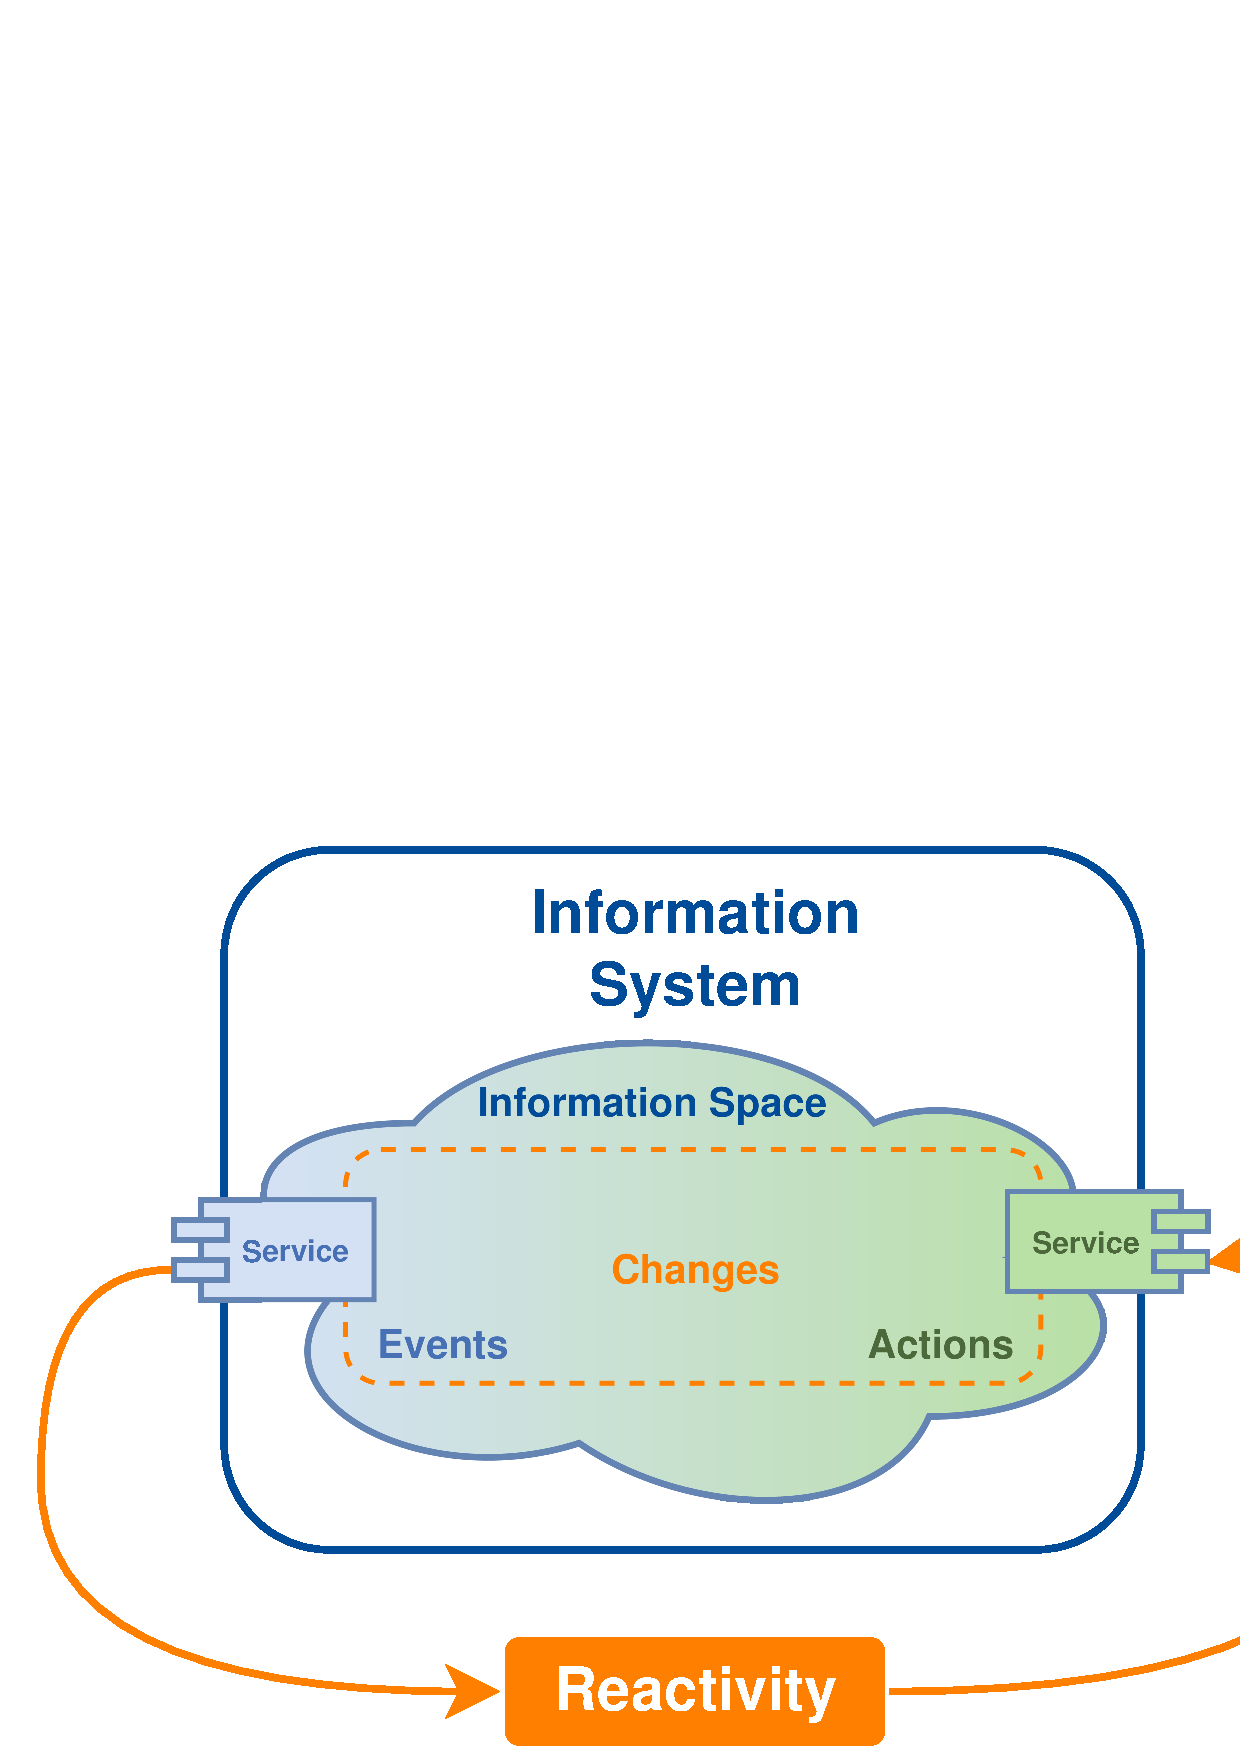
\includegraphics[width=0.7\textwidth]{figures/IS_InformationSpace}
  \caption{Reactivity imposed on \textrm{\glspl{infosystem}} and their \textrm{\glspl{infospace}} over Services}
  \label{fig:IS_InformationSpace}
\end{figure}
Data changes within an \textrm{\gls{infosystem}} can be detected and imposed from the outside, if apropriate interfaces to the services exist.
We model the detection of data changes as events, and the imposition of such changes as actions, as shown in Figure \ref{fig:IS_InformationSpace}.
Through this we are able to introduce an event-based model that is capable to detect events and react on behalf of them by imposing actions on any \textrm{\gls{infospace}}, be it the event origin or another one.
A more precise distinction of the required modules for such a reactivity imposing entity is displayed in Figure \ref{fig:Standard-Model-Template}, and each module is introduced in this chapter.
\begin{figure}[!ht]
  \centering
  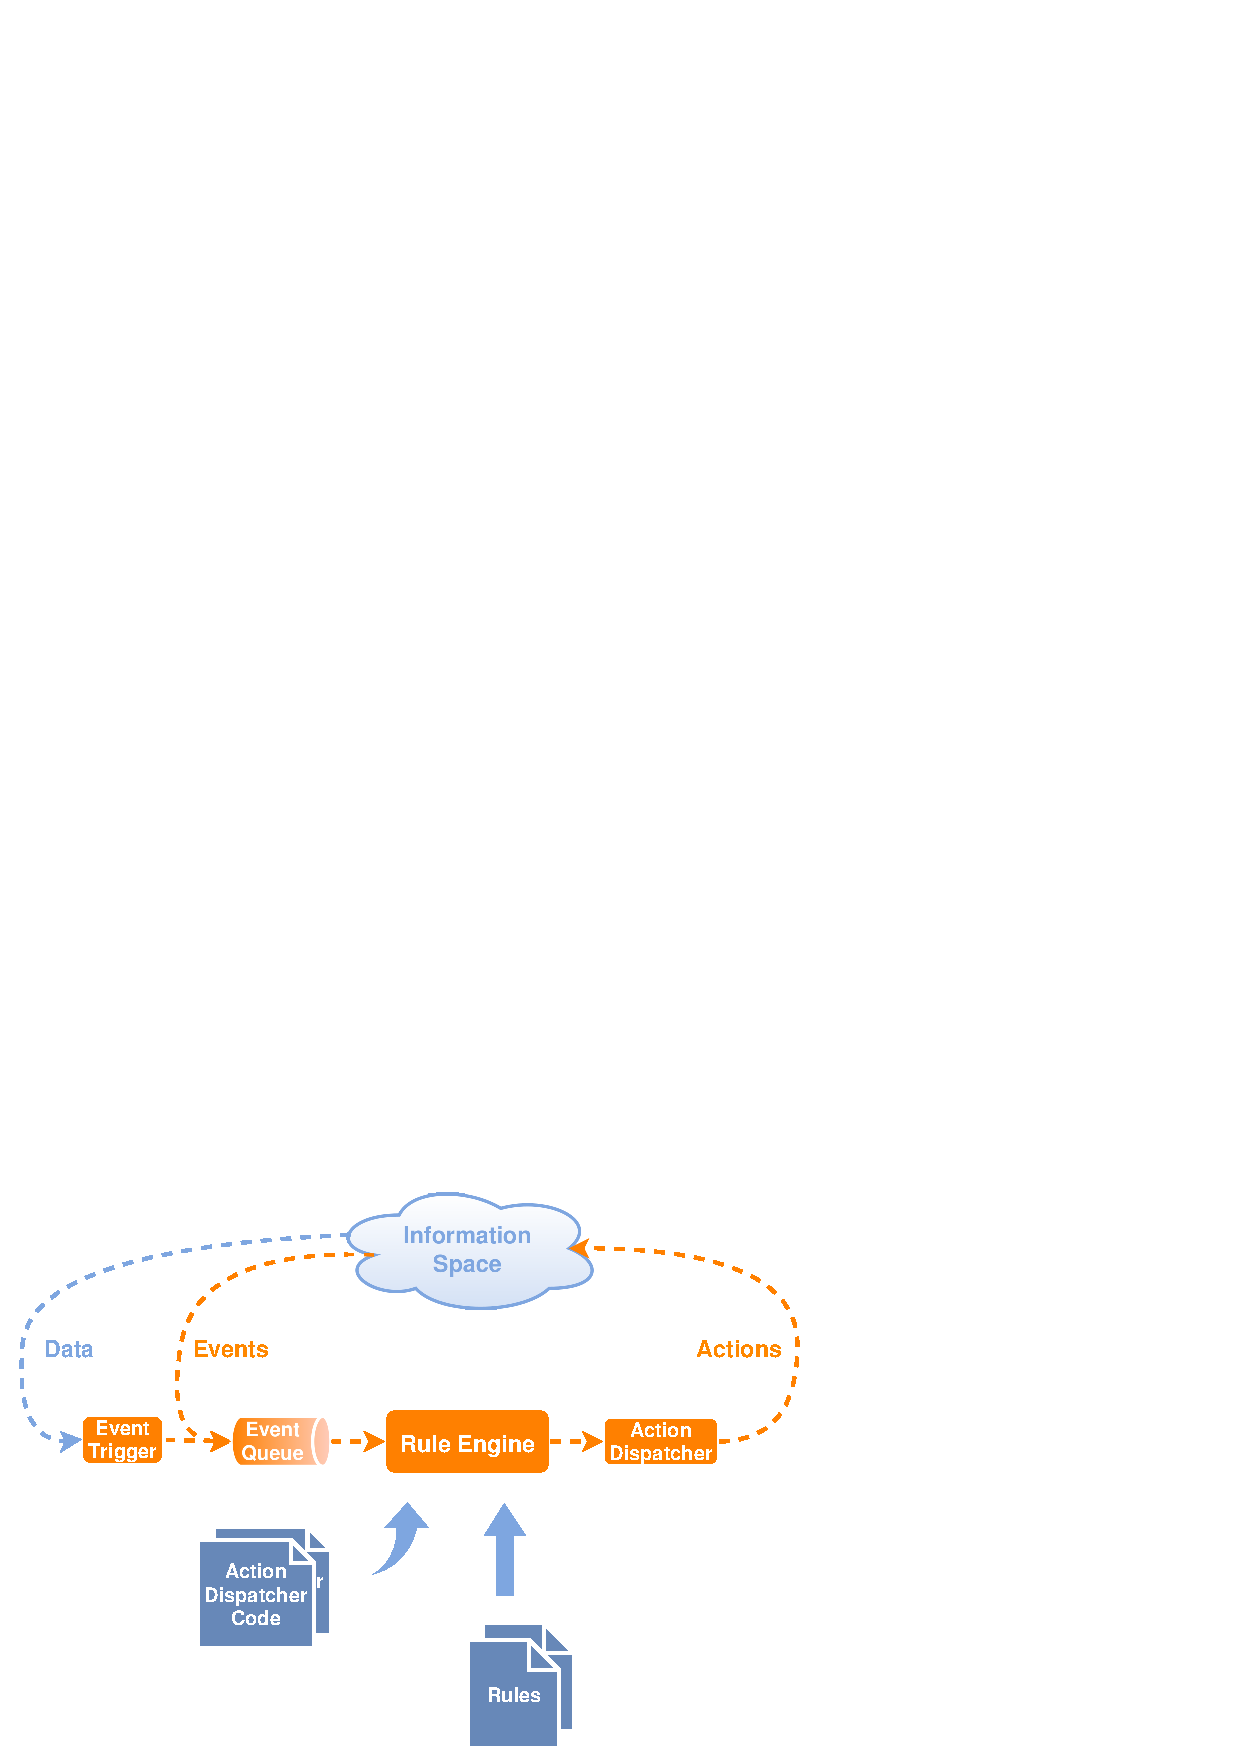
\includegraphics[width=0.7\textwidth]{figures/Standard-Model-Template}
  \caption{Conceptual Model for Reactive Information Systems and their Services}
  \label{fig:Standard-Model-Template}
\end{figure}



\section{From Physical Events to Virtual Events}
We introduced the \textrm{\gls{webofthings}} in the last chapter, where smart devices gain access to the Web.
It is based on the \textrm{Internet of Things} which dealt with the incorporation of sensor networks into the Internet on the network level.
Such sensors bring the physical world directly into the virtual world.
This transformation pictures an important difference between physical and virtual events.
In physics, and in particular relativity, an event indicates a physical situation or occurrence, located at a specific point in space and time.
While physical events correspond to a physical situation which is located at a specific point in space and time, virtual events primarily consist of implicit parameters, i.e. a name and occurrence time.
These virtual events can be anywhere within \textrm{\glspl{infosystem}} at any point in time and thus their actual location differs most certainly from its occurrence location.
But virtual events also have explicit parameters which correspond to all available information about the event, such as the origin.
As soon as events are transformed into the virtual world, the afore mentioned location information is transformed into explicit event parameters.
Therefore wherever a virtual event is, it has a name, an occurrence time and most likely some explicit parameters attached to it.
If the virtual event is of a physical nature, it has a physical location, if it is of a virtual nature, it is likely associated with a virtual origin.
Since in our model events are changes in data of an \textrm{\gls{infospace}}, they can be virtually anything, e.g. physical measurements, changes on a static webpage, changes of the object behind a \textrm{\gls{webservice}} or also a login attempt.
% TODO TABELLE Ort/Kultur(fussball/Apple, weltweit)/Saisonal(kalender)/Internet (ortlos, github)
% ceremony
% competition
% meeting
% disaster
% event horizon
% extinction event
% festival
% grouped events
% happening
% impact evetn
% media event
% mental event
% news
% party
% phenomenon
% sporting event
% synchronization


\section{Capturing Events from Information Systems}
The optimal case for an event-driven system which requires events from a remote \textrm{\gls{infosystem}} is, that events are triggered within the remote \textrm{\glspl{infosystem}} and then immediately communicated to interested parties, such as our envisioned reactivity imposing system.
But our research has shown that such \textrm{\glspl{infosystem}} are often passive and rarely provide ways for external systems to announce interest in changes of their data.
For example in the context of \textrm{\glspl{webresource}}, many of them provide access to their data over services, but do not actively communicate changes to interested parties.
This is where the upcoming concept of \textrm{\glspl{webhook}} comes into play.
Only through them we are able to provide real-time reactivity without risking huge costs of continuously polling for changes over all \textrm{\glspl{infospace}}.
%TODO future work?
We envision a future where the whole Web is event-driven and events are directed to any \textrm{\gls{infosystem}}, which is interested in them.
This would be the optimal case for effective real-time notifications and thus reactivity on the Web.
Since this in general not the case yet, we need to incorporate polling for changes into our model, in order to cope for the widely spread passiveness of \textrm{\glspl{infosystem}}.
Wherever an \textrm{\gls{infosystem}} is not capable to provide events to external \textrm{\glspl{infosystem}}, we can still read all the accessible data and detect changes in it, model them as events and feed them into our model.
In our model the polling for changes is incorporated in the \textrm{Event Trigger} modules.
Those are flexible modules that have the proper tools to access any \textrm{\gls{infosystem}} service and therefore its \textrm{\gls{infospace}} and are capable of identifying changes in the data.
For example the \textrm{\gls{www}}, as envisioned by Tim Berners-Lee\cite{DBLP:journals/en/Berners-LeeCGP92}, is an information universe of interlinked documents, that a user can browse through.
Through our model, we can pull changes in the data on the \textrm{\gls{www}}, i.e. document changes, and turn them into events.
These events which are derived from changes in the data of \textrm{\gls{infosystem}} are then fed into the \textrm{Event Listener}.
The \textrm{Event Listener} also pulls events directly from the \textrm{\glspl{infosystem}} that offers service functions which represent events but still need to be requested actively, e.g. new mail in inbox.



\section{Event Pattern Detection}
Traditional \textrm{\acrshort{eca}} systems only react on single events, but this might often not be enough to detect meaningful situations.
Primitive events occur at a point in time (e.g. a press down mouse button event).
When they are composed (e.g. the latter event with a release mouse button event), they turn into a composite event which is more complex and also has a duration.
Such a temporal event composition yields the chance to detect meaningful situations out of primitive events and react on them.
This is why there is a trend towards the detection of complex event patterns, as we have pointed out in the last chapter.
\textrm{\acrshort{cep}} could be incorporated into the rules of the \textrm{Rule Engine}, which then reacts on event patterns, but this opposes our vision of a successively growing complexity of composite events that are defined on top of each other and fed back into the \textrm{Event Listener}.
Thus in our model an \textrm{Event Composition} module composes events into more complex events according to \textrm{\acrshort{ced}} definitions.
It is a very active research field, it has seen interesting studies\cite{akdere2008plan}\cite{2004_1265833} and outcomes\footnote{such as http://drools.jboss.org/drools-fusion.html} that could be incorporated into our model.
Such an event composing service systems works loosely coupled an could be realized by any suitable system, as described in \cite{robins2010complex}.



\section{Imposing Reactivity to Information Spaces}
In the last chapter we gave an introduction into reactivity and the \textrm{\acrshort{eca}} paradigm as an approach to achieve it.
So far we have introduced the first part of our model which provides the foundation of an \textrm{\acrlong{eda}}.
What we also need is a module that translates events into actions on \textrm{\glspl{infosystem}}.
Almost all existing \textrm{\acrshort{eca}} system's actions write on the local \textrm{\gls{infospace}} which opposes our vision of the orchestration of different \textrm{\glspl{infosystem}} in order to impose reactivity on top or between them.
For that reason we introduce the \textrm{Action Dispatcher} modules which are located right behind the \textrm{Rule Engine} in terms of the data flow and complete the reactivity flow between heterogeneous \textrm{\glspl{infosystem}}.
\textrm{Action Dispatcher} modules are an important part of our model because they allow flexible coupling with \textrm{\gls{infosystem}} services, much like the \textrm{Event Trigger} modules do.
\textrm{Event Trigger} and \textrm{Action Dispatcher} modules are communication abstractions to services of \textrm{\glspl{infosystem}}, that allow us to deal with their heterogeneity in terms of communication.
The \textrm{\gls{infospace}} of an \textrm{\gls{infosystem}} is not limited to internal data, but can also refer to a coupling with other devices and the sensing and controlling of it.
Thinking of the \textrm{\gls{webofthings}} this can also include an \textrm{Action Dispatcher} that has access to an \textrm{\gls{infosystem}} which controls devices and thus is capable of turning down the heating in a house, as shown in Figure \ref{fig:InformationSystemWoT}.
\begin{figure}[!ht]
  \centering
  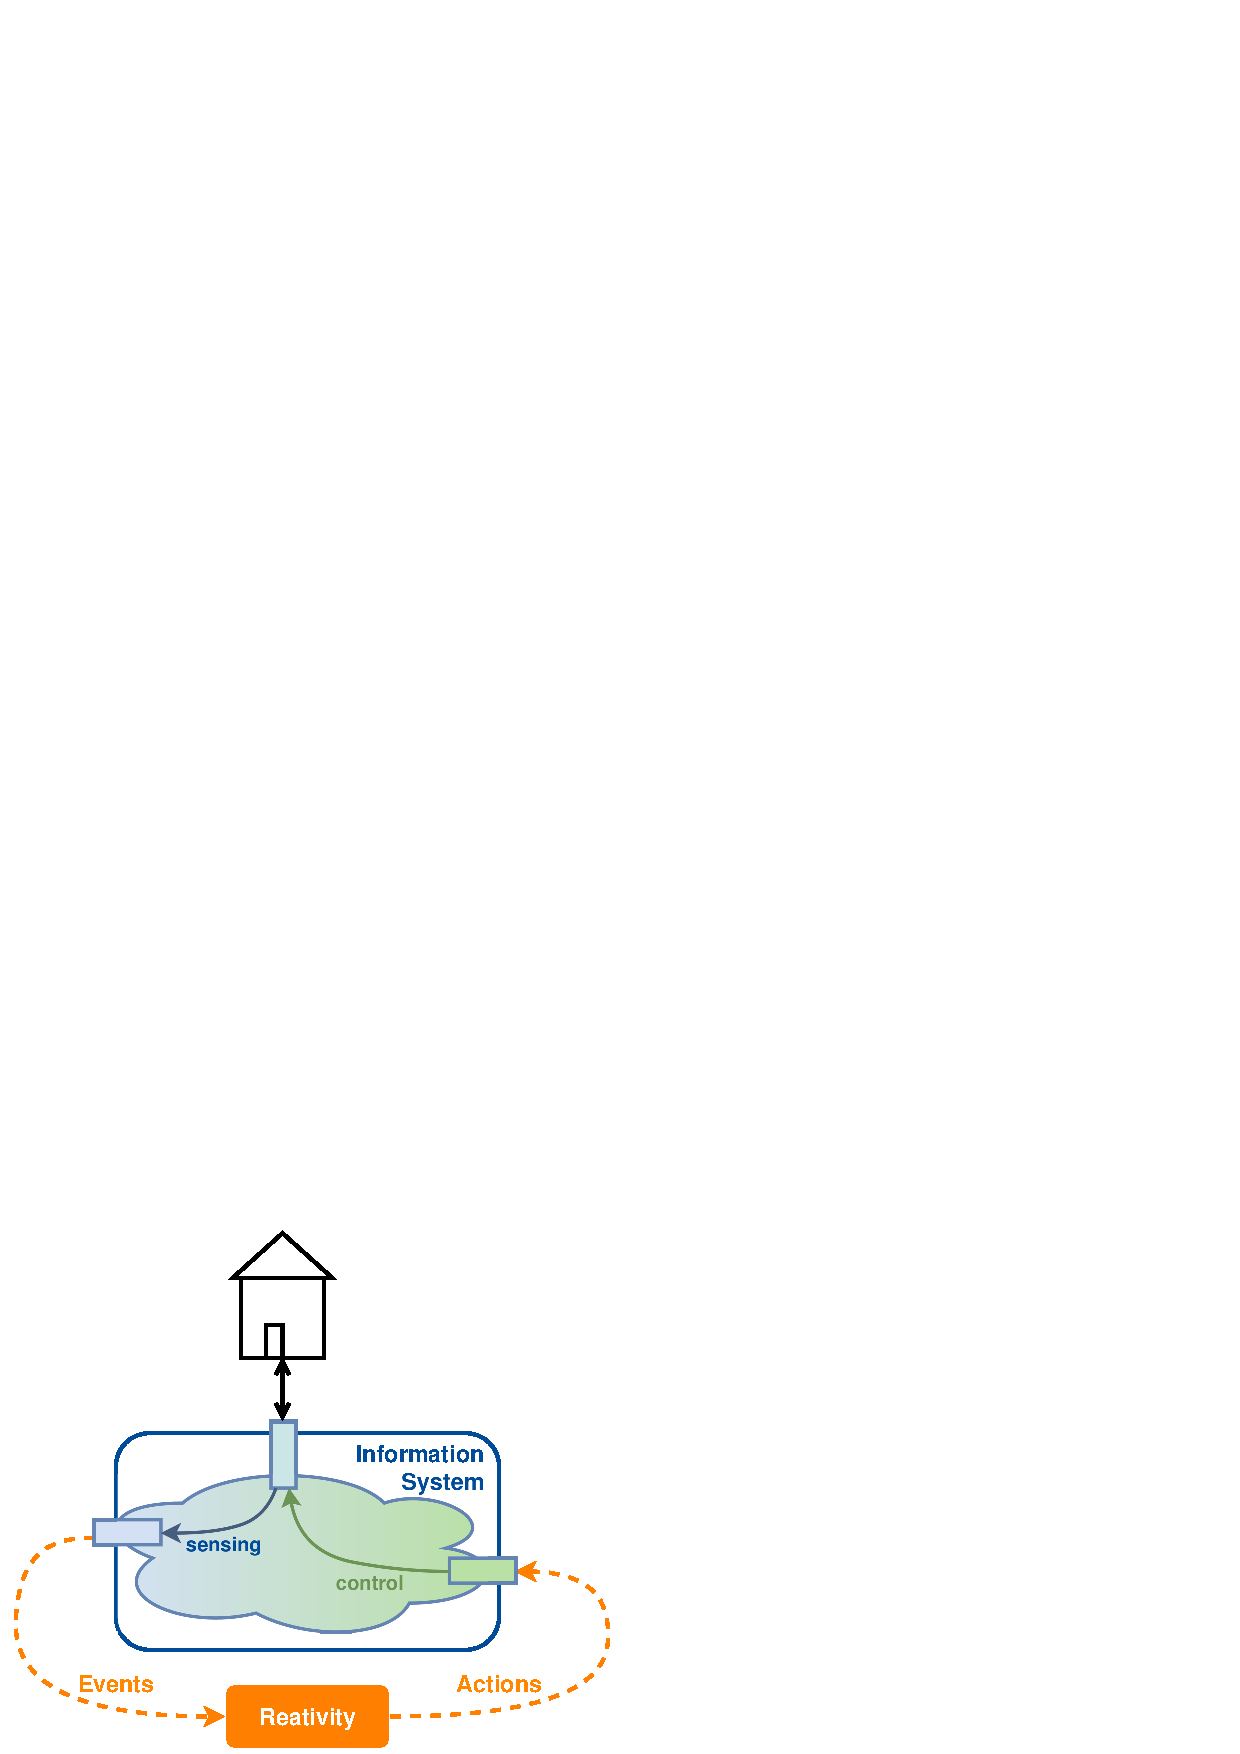
\includegraphics[width=0.6\textwidth]{figures/InformationSystemWoT}
  \caption{\textrm{\glspl{infosystem}} providing access to the \textrm{\gls{webofthings}} over their Services}
  \label{fig:InformationSystemWoT}
\end{figure}

So far we defined all the modules to access \textrm{\glspl{infosystem}} over their services, therefore we are able to define a \textrm{Rule Engine} that orchestrates them in a reactive way.
We have shown in the last chapter that \textrm{\acrshort{eca}} rules consist of three parts; an event to be recognized, conditions to be evaluated on the event and actions to be executed if an event triggers the rule through valid conditions.


% FIXME something on rules angine missing???


% EARTH QUAKE example

% Different points on earth's surface would feel the earthquake, which originates from the same epicentre, at a different point in time with a different intensity.
% A Web event model of an earthquake would consist of a large number of identical \textrm{\textbf{ground-shake}} events that occur at different points in time and places.
% Therefore they would hold different spatial location informations and intensities.
% These events can be thought of as emitted into the Web by a seismometer sitting at the corresponding location.
% \begin{figure}[!ht]
%   \centering
%   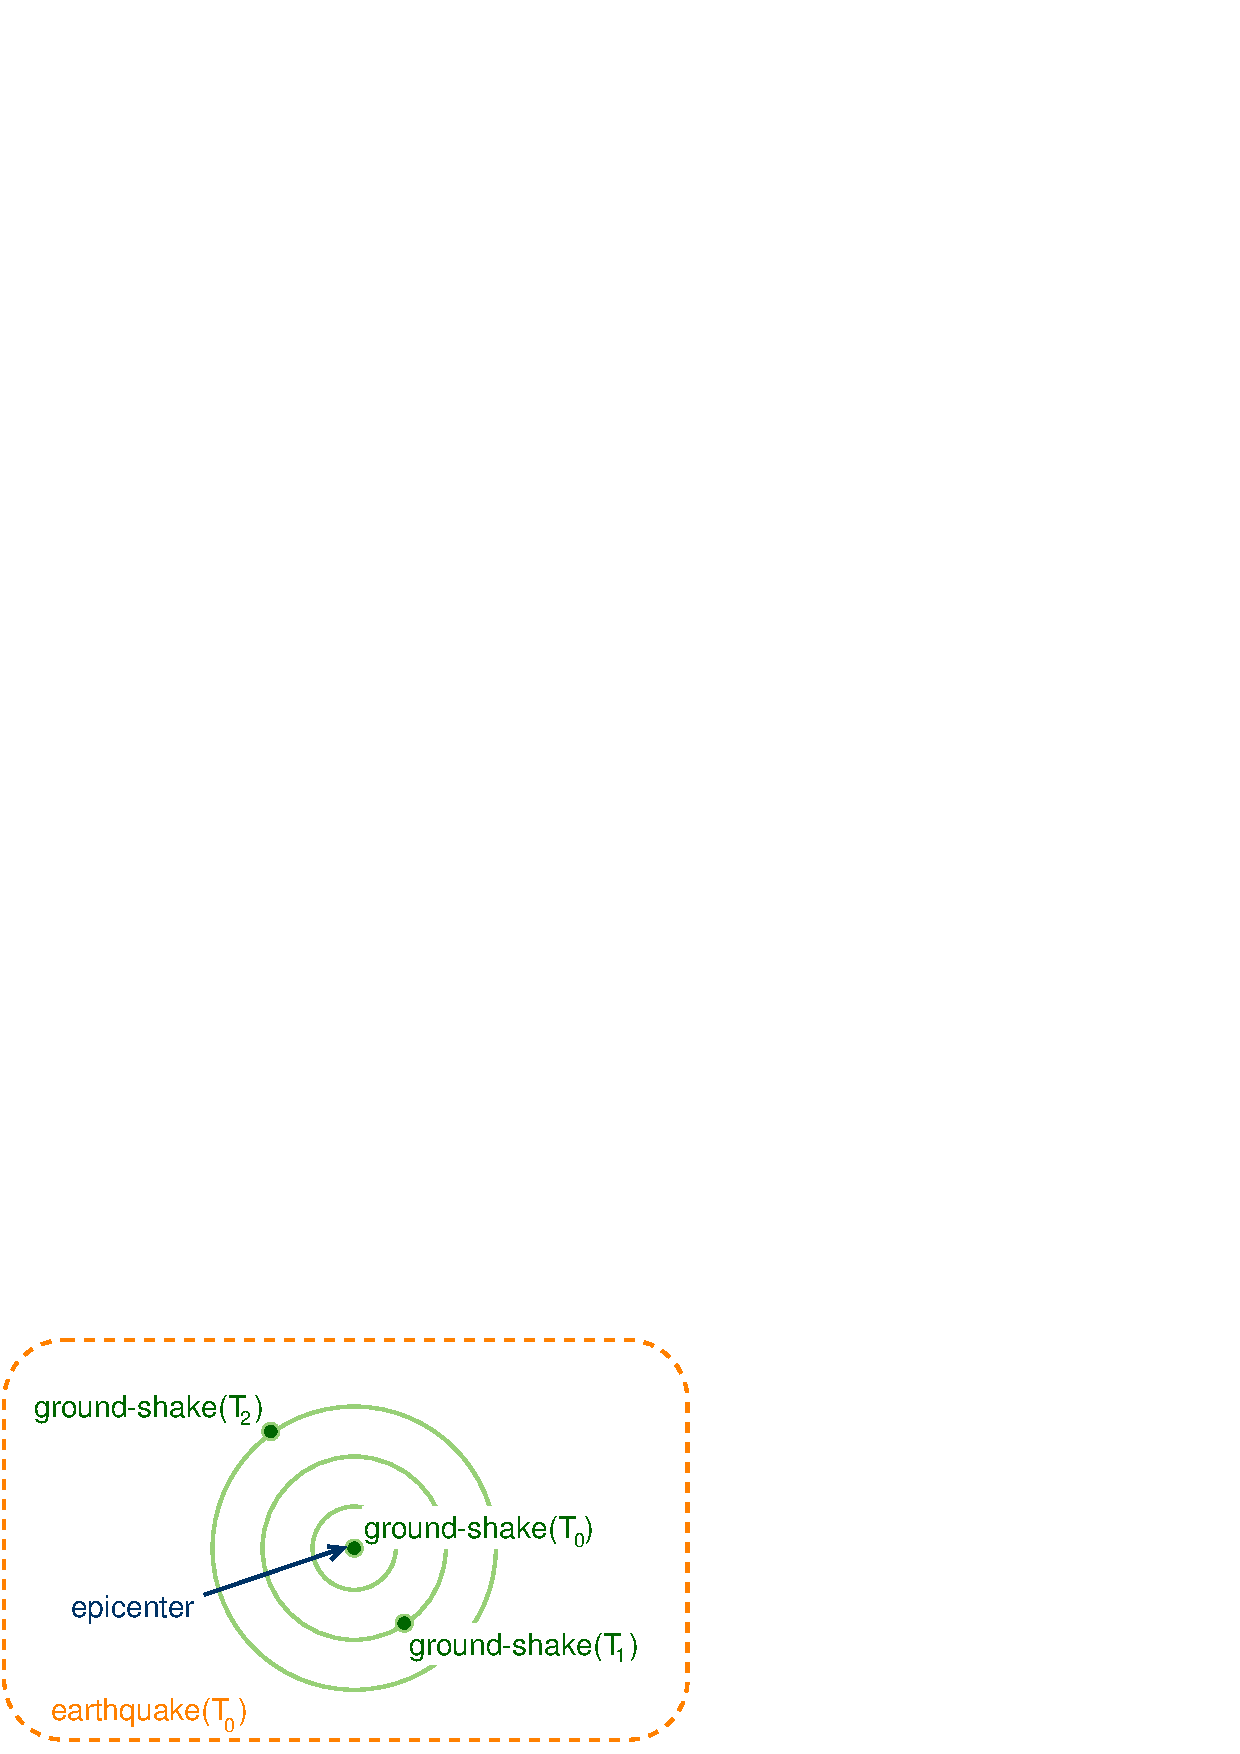
\includegraphics[width=0.6\textwidth]{figures/Earthquake}
%   \caption{Web Event Model of an Earthquake}
%   \label{fig:Earthquake}
% \end{figure}
% Within the Web, events lose their tight coupling to locations and retain only a time component.
% The event instances keep this information as descriptive metadata.
% A reactive system such as we envision it, could detect these \textrm{\textbf{ground-shake}} events and react on behalf of each one of them.
% Because of the Web's latency these events do most certainly not arrive at systems within the Web in the original order, in which they were triggered.
% They also do most likely not arrive in the exact same order for all systems.
% This leaves us with time as the only important factor left, to distinguish events from each other in the first place.
% To get an earthquake event out of all these ground shaking informations floating through the Web, somebody would need a reactive system that detects these events and assembles them into one earthquake event, together with a computed epicentre and magnitude.
% Such a system (we call it \textrm{\textbf{earthquake-tracker}}) would own an earthquake model that allows it to decide whether a \textrm{\textbf{ground-shake}} event belongs to one physical earthquake or to another one, depending on its spatial location information and the intensity at that point in time.
% It could then emit a more complex \textrm{\textbf{earthquake}} event (with epicentre and magnitude) that allows other systems to interpret this physical event and react on behalf of it.

% Let's take another system that reacts on a physical earthquake.
% It is now left with a multitude of different options on how to react.
% It could only react on the \textrm{\textbf{earthquake}} event which is coming from the system above (\textrm{\textbf{earthquake-tracker}}) that applies its earthquake model to the incoming \textrm{\textbf{ground-shake}} events.
% But how long will it take for this system to deploy its \textrm{\textbf{earthquake}} event?
% Eventually it waits for one round-trip of a seismic wave around the world, which takes approximately half an hour.
% What if it waits two or three round-trip times in order to collect more accurate data?
% And what if our new system wants to react as fast as possible in order to warn people all around the world.
% It would then need to react on a small subset of the \textrm{\textbf{ground-shake}} events in order to quickly identify a real earthquake and take measurements, e.g. immediately send out text messages to people, or to deploy yet another ( this time \textrm{\textbf{earthquake-alert}}) event into the Web's \textrm{\gls{infospace}}.
% This relatively simple example discloses the complex nature of event-driven systems, but also their high flexibility and fine grained tuning possibilities.
